% ============================================================
% APPENDIX TEMPLATE (team-final template only)
% Replace the placeholder text below with supplementary material.
% Sections are lettered (A, B, ...); figures, tables and equations are
% numbered within each appendix section (Table A.1, Figure B.1, (A.1)).
% All numbers are placeholders, NOT experimental results.
% ============================================================
\ogbeginappendix

\section{Implementation Details}
\label{app:details}

Use this appendix section for implementation details that do not fit in the
main text. Table~\ref{tab:app-hparams} shows how a hyperparameter table is
typeset; floats in the appendix are numbered per section.

\begin{table}[!htbp]
  \centering
  \footnotesize
  \caption{Placeholder hyperparameters. Replace the settings and values with
  those of your report. \textbf{All values are placeholders.}}
  \label{tab:app-hparams}
  \begin{tabularx}{\linewidth}{>{\raggedright\arraybackslash}Xccc}
    \toprule
    Setting & Stage 1 & Stage 2 & Stage 3 \\
    \midrule
    Learning rate     & $2\times10^{-5}$ & $1\times10^{-5}$ & $5\times10^{-6}$ \\
    Global batch size & 256  & 128  & 64   \\
    Training steps    & 8k   & 4k   & 1k   \\
    Weight $\lambda$  & ---  & 0.1  & 0.1  \\
    \bottomrule
  \end{tabularx}
\end{table}

\subsection{Additional Formulation}

Equations in the appendix are numbered within the section, for example
\begin{equation}
  \hat{\mathbf{h}} = \frac{\mathbf{h} - \mu}{\sigma + \epsilon},
  \label{eq:app-norm}
\end{equation}
where $\mu$ and $\sigma$ are placeholder statistics and $\epsilon$ is a small
constant (Equation~\eqref{eq:app-norm}).

\subsection{Reproducibility Checklist}

\begin{itemize}[leftmargin=1.2em,itemsep=1pt,topsep=2pt]
  \item Code and configuration files: \url{https://github.com/isjinghao/OralGPT}.
  \item Model weights and datasets: \url{https://huggingface.co/OralGPT}.
  \item Hardware, software versions and random seeds: \textit{placeholder}.
\end{itemize}

\section{Additional Results}
\label{app:results}

Use this section for additional tables, figures and qualitative examples.
Figure~\ref{fig:app-results} shows how an appendix figure is numbered, and
Appendix~\ref{app:details} can be cross-referenced in the usual way.

\begin{figure}[!htbp]
  \centering
  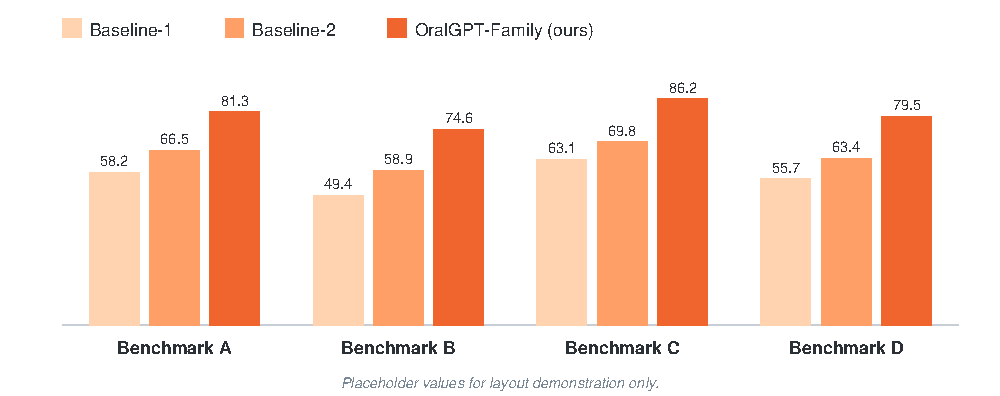
\includegraphics[width=0.75\linewidth]{assets/fig_results.pdf}
  \caption{Placeholder additional results. Replace this figure with
  supplementary results; the values shown are placeholders.}
  \label{fig:app-results}
\end{figure}
